\section{Resultados finales y experimentación}

{\centering
    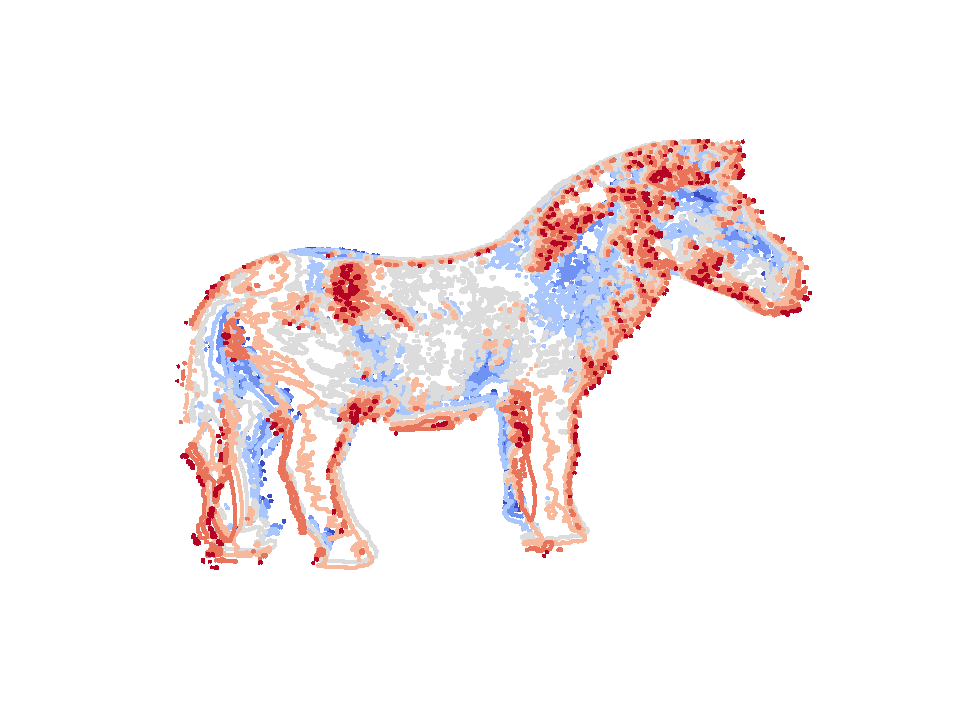
\includegraphics[scale=0.6]{informe/imagenes/supnivel/supNivelCaballoLucesPropias578N1.pdf} \\
}
{\centering
    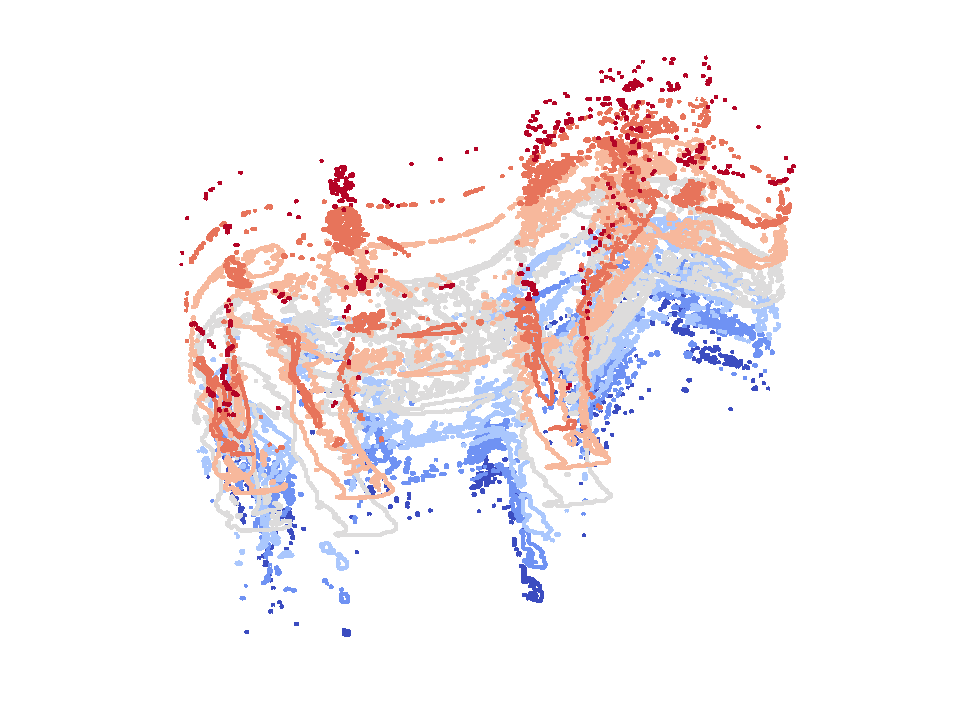
\includegraphics[scale=0.6]{informe/imagenes/supnivel/supNivelCaballoLucesPropias578N2.pdf} \\
}
{\centering
    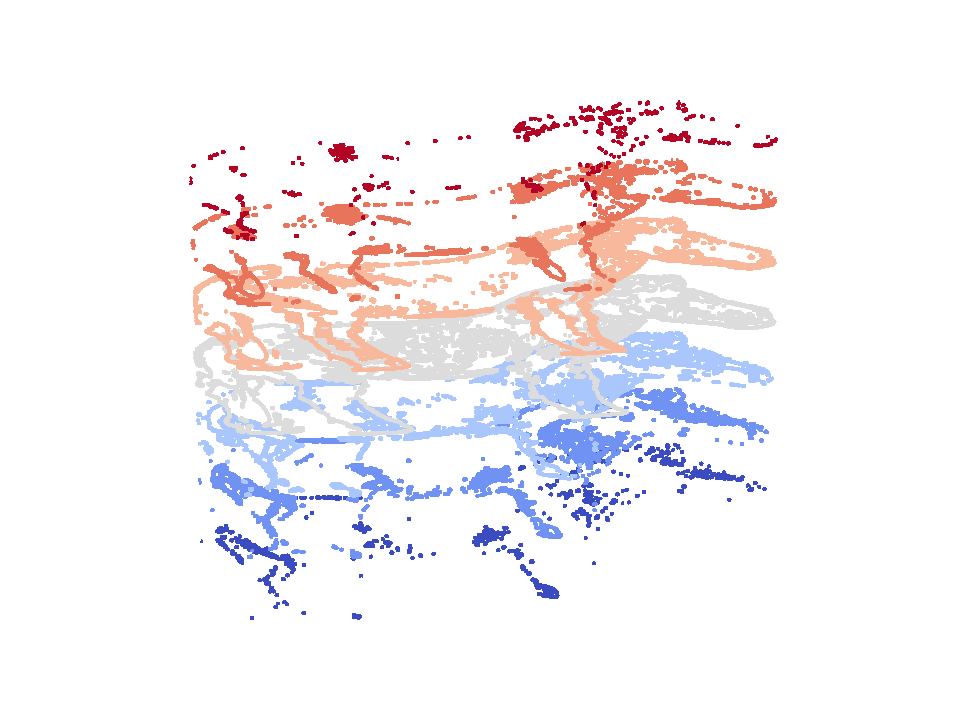
\includegraphics[scale=0.6]{informe/imagenes/supnivel/supNivelCaballoLucesPropias578N3.pdf}
    \captionof{figure}{Curvas de nivel de la función de profundidad (para cada píxel, su profundidad estimada) Los valores fueron calculados utilizando las luces que obtuvimos en nuestra calibración.}
}

\newpage
Si bien esperábamos obtener una superficie mucho mas \textit{suave}, creemos que los resultados fueron satisfactorios. Puede observarse perfectamente en los gráficos de curvas de nivel de arriba que en cada píxel la profundidad estimada es adecuada y se corresponde con la iluminación de las fotos originales. Veamos una representación de la función de profundidad con los mismos datos en un modelado 3D:

{\centering
    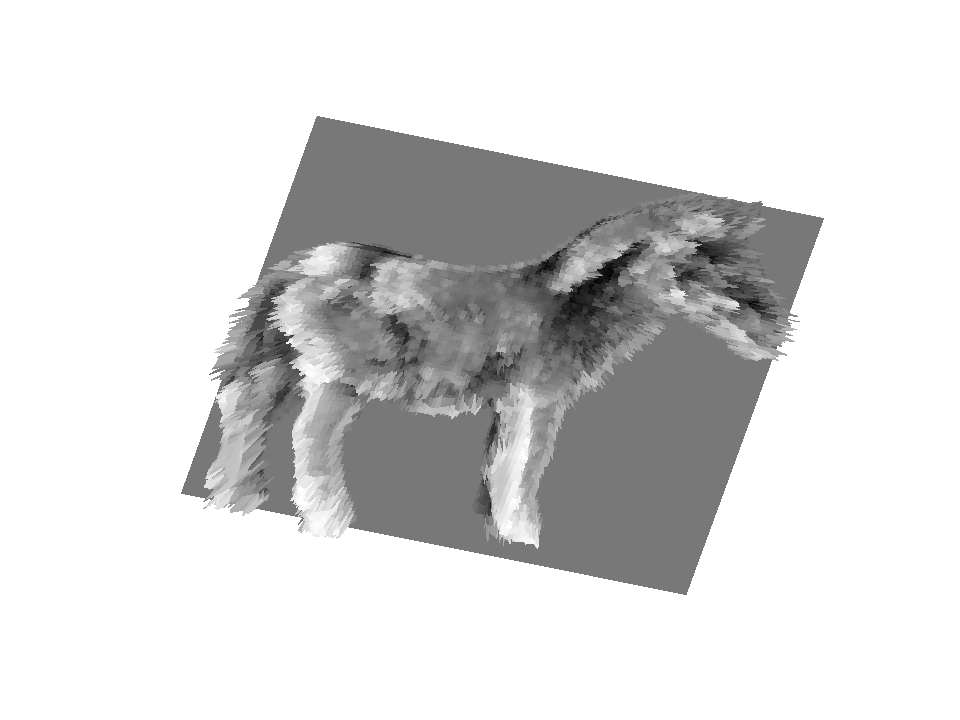
\includegraphics[scale=0.8]{informe/imagenes/profundidades/profundidadesCaballoLucesPropias578.pdf} \\
    \captionof{figure}{Profundidades calculadas con luces propias, 5, 7, 8}
}

$ $\newline
En la imagen de arriba podemos ver lo que mencionamos sobre la \textit{suavidad} de la superficie. Es claro que es diferente a lo visto en la imagen de ejemplo del enunciado, pero incluso así son distinguibles las alturas de los diferentes píxeles. El \textit{fondo} del modelo es un plano perfecto por el hecho de haber utilizado la máscara para no realizar cálculos innecesarios. Sospechamos que los picos tiene que ver con la forma en que aproximamos los planos tangentes.\\

Veamos que obtenemos si partimos directamente de las \textbf{normales} provistas por la cátedra:

{\centering
    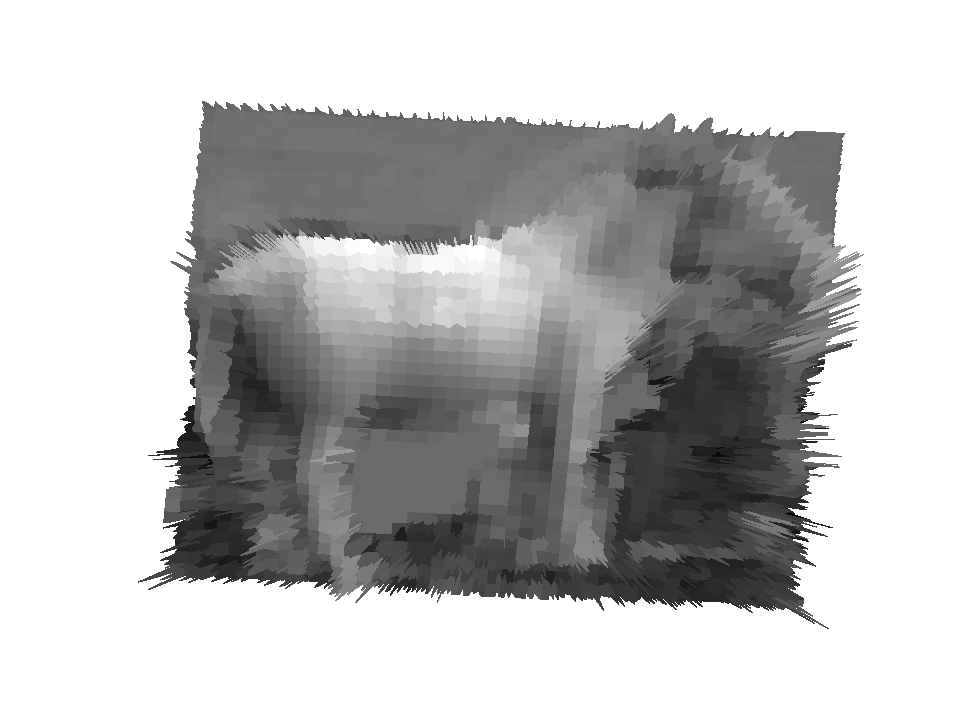
\includegraphics[scale=0.7]{informe/imagenes/profundidadesCaballoNormalescatedra.pdf} \\
}

Si bien las luces con las que fueron obtenidas las normales de la cátedra son desconocidas para nosotros, podemos hacer algunas comparaciones. Aunque esté llena de \textit{picos}, sobretodo en los bordes, parece ser una superficie un poco mas suave que la obtenida por nosotros. Dado que no sabemos cuales fueron las luces utilizadas en el cálculo, no podemos descartar que sea un tema de elección de luces. Sin embargo, incluso aunque fuesen las mismas, veremos mas adelante que lo calibrado por nosotros no se corresponde en un 100\% por lo que es esperable que se observen diferencias. \\

Otra cosa a notar, es que en ambas los detalles del rostro del caballo se pierden. Si bien era esperable ya que son áreas delicadas, nos dá la pauta de que nuestras aproximaciones pueden no ser del todo correctas. De todos modos, no podemos saber si en una estimación 'bien hecha' los detalles se mantienen o no. \\

Realizamos los cálculos de profundidad con una imagen que tiene más detalles, para ver si sucede lo mismo que con el rostro del caballo. La siguiente es un gráfico con las profundidades de Buda, con las luces $0, 1$ y $2$ calibradas por nosotros.

{\centering
    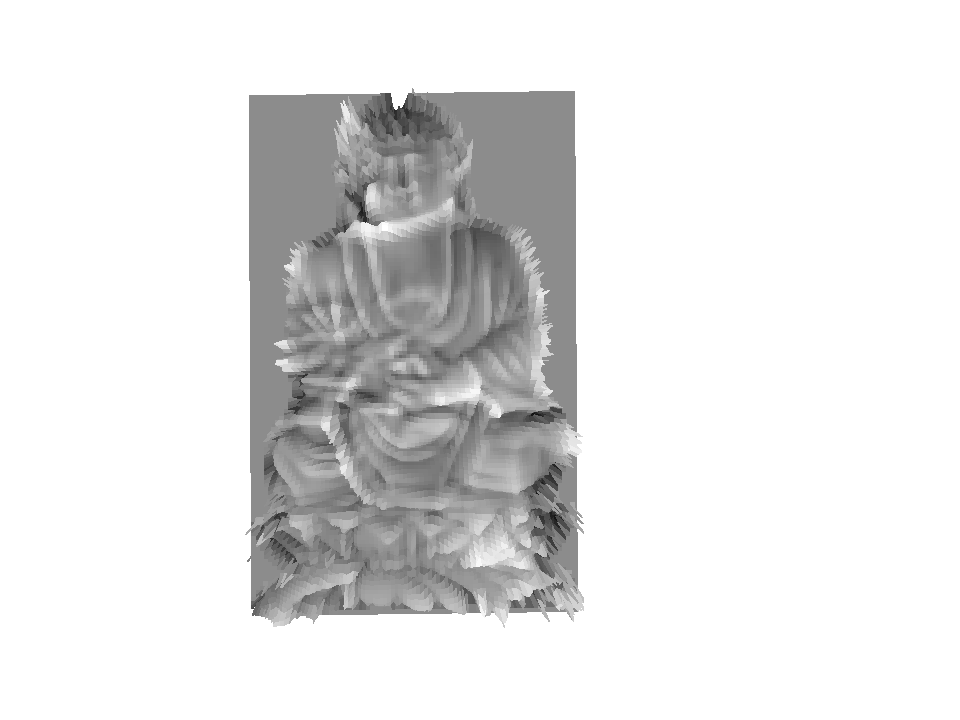
\includegraphics[scale=0.8]{informe/imagenes/profundidades/profundidadesBudaLucesPropias012.pdf} \\
}

Los detalles del cuerpo se mantuvieron bastante bien, y el área central e inferior tiene mas suavidad que la que habíamos logrado con la anterior imagen. En los bordes nuevamente tenemos picos, se deben a la diferencia brusca que hay con el plano. Es interesante notar que se produjo una deformación en el sector superior, creemos que tiene que ver con la gran cantidad de cambios de luz en un área tan pequeña. \\


% 1. Comparar las direcciones de iluminacion obtenidas por el metodo de calibracion con las provistas por la catedra \\
\newpage
Mencionamos anteriormente que se encontraron diferencias entre las luces calibradas por nosotros y las luces  de la cátedra. Veamos los resultados que obtuvimos. En general, niguna luz quedó \textit{exactamente} igual, pero sí quedaron similares. \\

Dado que es complicado visulizar diferencias entre vectores tridimensionales, analizaremos por un lado el eje $z$ y por el otro los ejes $x$ e $y$. En el siguiente gráfico tomamos para cada luz, los ejes $z$ y calculamos su diferencia. \\

{\centering
    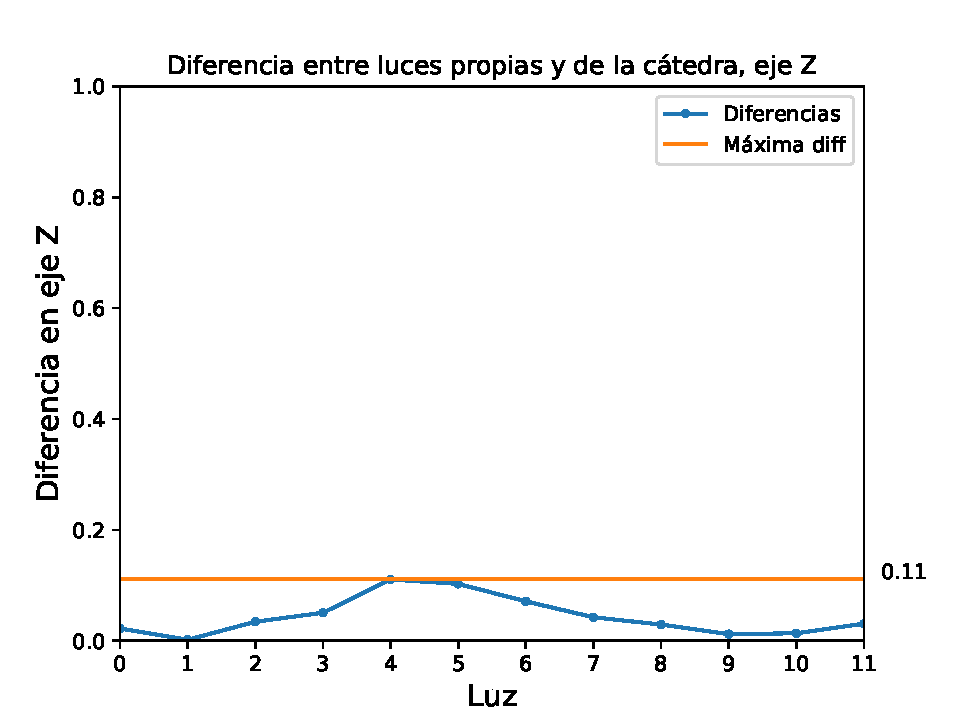
\includegraphics[scale=0.7]{informe/imagenes/lucesEjezDiferencias.pdf} \\
}

Podemos observar que la la diferencia máxima es aproximadamente $0.1$ mientras que la diferencia mínima está cercana a cero (es exactamente $0.001821$ en la luz $1$). Creemos que si bien no es perfecto, es una diferencia aceptable. Dado que todos los vectores son unitarios (pues fueron normalizados) es lógico esperar diferencias entre los ejes x e y. A continuación puede verse el gráfico resultante. Las luces que se corresponden con las propias y las de la cátedra están señaladas con el mismo color. \\

Podemos observar que si bien las diferencias son notorias, todas se encuentran en el mismo rango en inclinación. No hay ninguna que haga cosas extrañas como apuntar en sentido inverso. Creemos que las diferencias no afectarán demasiado el resultado final.

{\centering
    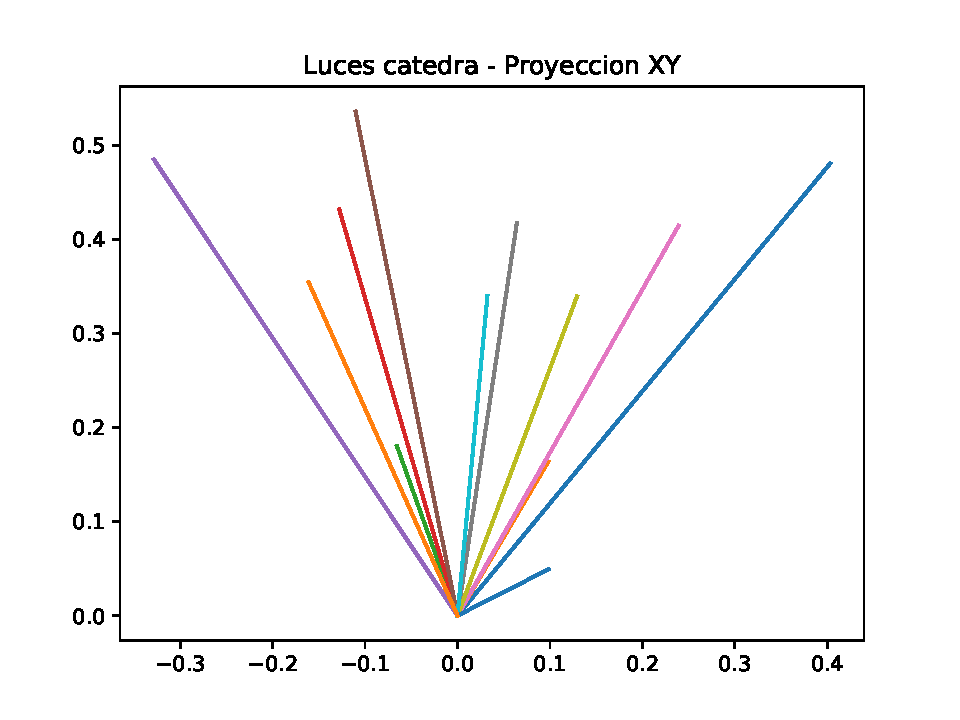
\includegraphics[scale=0.8]{informe/imagenes/lucesCatedraProyeccionXY.pdf} \\
    % \captionof{figure}{Luces de la cátedra en la proyección x,y}
}
{\centering
    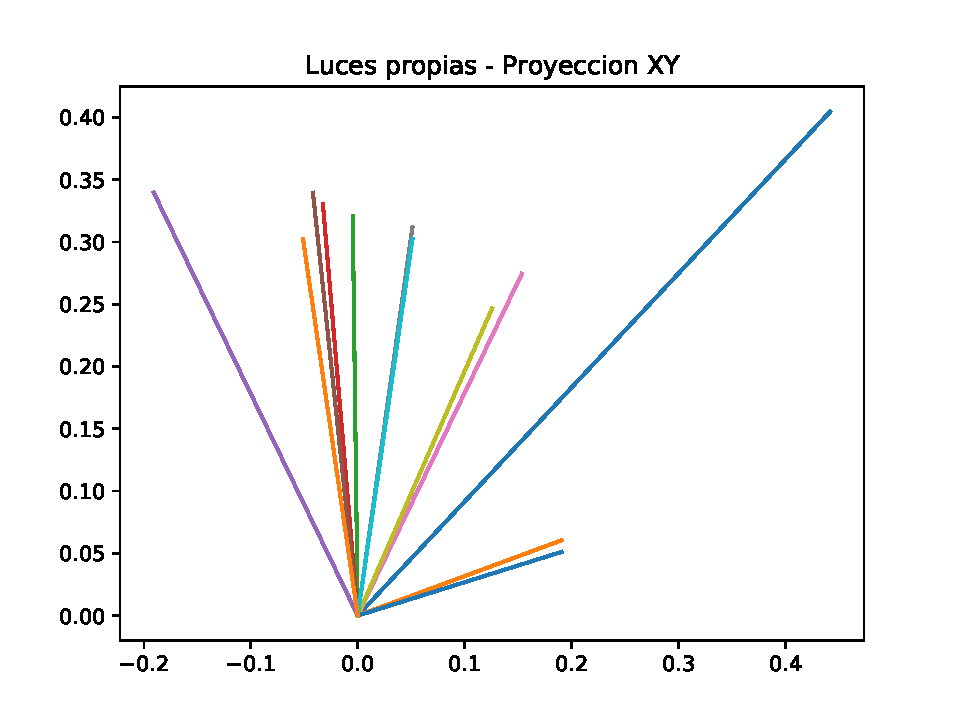
\includegraphics[scale=0.8]{informe/imagenes/lucesPropiasProyeccionXY.pdf} \\
    % \captionof{figure}{Luces propias en la proyección x,y}
}

$ $\newline

% 2. Como afecta la calibracion del sistema en el resto de las etapas \\

Dado que las luces son utilizadas para el cálculo de las normales, queremos ver cómo nos afecta la calibración en esta etapa. Para eso, resolveremos el sistema de ecuaciones y guardaremos los vectores normales obtenidos. Como las mayores diferencias entre luces podían verse en los ejes $x, y$ estos ejes serán los que usaremos en la comparación. \\

En los gráficos que se encuentran a continuación, para cada píxel se grafica un vector que corresponde a la normal en ese punto. Como son \textit{miles} de normales, puede dar la impresión de que se grafican puntos pero no es así: son los vectores en forma de 'flechas'. \\

En todos los gráficos se utiliza exactamente la misma área de la imagen para que sean comparables. Para la resolución del sistema que calcula las normales se ultiliza eliminación gaussiana con pivoteo parcial para tratar de minimizar el error numérico. Para el primer experimento tomaremos nuestra 'mejor luz', la $1$ junto con las luces $4$ y $5$ que parecen ser las 'peores'. Esperábamos obtener malos resultados ya que dos luces no eran buenas, sin embargo los resultados fueron bastante buenos. \\

Las diferencias mas notorias se encuentran en el ojo y en la oreja del caballo. Creemos que tiene que ver porque son las áreas con más detalle pero menor iluminación. Sin embargo, no creemos que sea una diferencia demasiado significativa.

% {\centering
%     \includegraphics[scale=0.5]{informe/imagenes/normales/normalesCaballoLucesPropias145.pdf} \\
%     \includegraphics[scale=0.5]{informe/imagenes/normales/normalesCaballoLucesCatedra145.pdf}
% }


\begin{figure}[H]
\centering
\begin{minipage}{.5\textwidth}
    \centering
        \includegraphics[scale=0.5]{informe/imagenes/normales/normalesCaballoLucesCatedra145.pdf}
    \captionof{figure}{Nomales con luces catedra: 1, 4, 5}
\end{minipage}%
\begin{minipage}{.5\textwidth}
    \centering
        \includegraphics[scale=0.5]{informe/imagenes/normales/normalesCaballoLucesPropias145.pdf} \\
    \captionof{figure}{Normales con luces propias: 1, 4, 5}
\end{minipage}
\end{figure}

Aprovecharemos las siguientes imágenes podremos observar dos cosas. La primera es ver un poco más sobre las diferencias entre las luces de la cátedra y las calculadas por nosotros, y lo segundo es como cambian las normales cuando se toma un set de luces diferentes. \\

En el siguiente caso no tomamos la luz número $1$, que era la mejor que teníamos y en su lugar tomamos otra de las 'malas'. En este caso, consideraremos las luces $4, 5$ y $6$. Podemos observar que tanto las de la cátedra como las propias son demasiado oscuras, sin embargo la nuestra lo es mucho más. Los rasgos faciales dejaron de apreciarse. \\

\begin{figure}[H]
\centering
\begin{minipage}{.5\textwidth}
    \centering
        \includegraphics[scale=0.5]{informe/imagenes/normales/normalesCaballoLucesCatedra456.pdf}
    \captionof{figure}{Nomales con luces catedra: 4, 5, 6}
\end{minipage}%
\begin{minipage}{.5\textwidth}
    \centering
        \includegraphics[scale=0.5]{informe/imagenes/normales/normalesCaballoLucesPropias456.pdf} \\
    \captionof{figure}{Normales con luces propias: 4, 5, 6}
\end{minipage}
\end{figure}

Al haber tomado otro set de luces, la forma general de la imagen no cambia demasiado, pero si hay bastante diferencia entre los rangos mas finos.

\todo[inline]{Continuar}
